\documentclass[crop, tikz]{standalone}
\usetikzlibrary{decorations.markings}

\usepackage{amsmath, amssymb}
\newcommand{\vx}{\boldsymbol{x}}
\newcommand{\vbeta}{\boldsymbol{\beta}}
\newcommand{\RR}{\mathbb{R}}
\newcommand{\va}{\boldsymbol{a}}
\newcommand{\vb}{\boldsymbol{b}}
\newcommand{\vW}{\boldsymbol{W}}
\newcommand{\vy}{\boldsymbol{y}}

\begin{document}
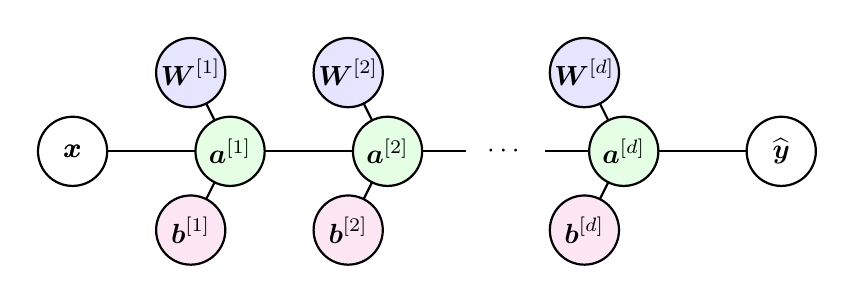
\begin{tikzpicture}
    \matrix[row sep=1em]
    {
        % % \begin{scope}[thick,decoration={markings, mark=at position 0.5 with {\arrow{latex}}}]
        % %     \draw[thick, postaction={decorate}] (0.5, 1)  -- (2, 0);
        % %     \draw[thick, fill=blue!15] (0.5, 1) node {$\beta_0$} circle (1em);
        % %     \node[above left] at (0.15, 1) {variable node};
        % %     \draw[thick, postaction={decorate}] (0, 0)  -- (2, 0);
        % %     \draw[thick, fill=yellow!15] (0, 0) node {$\vx$} circle (1em);
        % %     \node[above left] at (-0.35, 0) {input node};
        % %     \draw[thick, postaction={decorate}] (0.5, -1)  -- (2, 0);
        % %     \draw[thick, fill=blue!15] (0.5, -1) node {$\vbeta$} circle (1em);
        % %     \draw[thick, fill=green!15] (2, 0) node {$y$} circle (1em);
        % %     \node[above right] at (2.35, 0) {output node};
        % %     \node[below right] at (2.35, 0) {$y = \vbeta^T\vx$};
        % % \end{scope}; \\
        %     \draw[thick] (0, 0)  -- (2, 0);
        %     \draw[thick, fill=white] (0, 0) node {$\vx$} circle (1.25em);
        %     \node at (0, 0) {$\vx$};
        %     \foreach \i in {1, 2, 3} {
        %         \draw[thick] ({2*\i - 0.5}, 1)  -- (2*\i, 0);
        %         \draw[thick, fill=blue!10] ({2*\i - 0.5}, 1) node {$\vW^{[\i]}$} circle (1.25em);
        %         \draw[thick] (2*\i, 0)  -- ({2*\i + 2}, 0);
        %         \draw[thick] ({2*\i - 0.5}, -1)  -- (2*\i, 0);
        %         \draw[thick, fill=magenta!10] ({2*\i - 0.5}, -1) node {$\vb^{[\i]}$} circle (1.25em);
        %         \draw[thick, fill=green!10] (2*\i, 0) node {$\va^{[\i]}$} circle (1.25em);
        %     }
        %     \draw[thick, fill=white] (8, 0) node {$\vy$} circle (1.25em);
        %     \\
            \draw[thick] (0, 0)  -- (2, 0);
            \draw[thick, fill=white] (0, 0) node {$\vx$} circle (1.25em);
            \node at (0, 0) {$\vx$};
                
            \draw[thick] ({2*1 - 0.5}, 1)  -- (2*1, 0);
            \draw[thick, fill=blue!10] ({2*1 - 0.5}, 1) node {$\vW^{[1]}$} circle (1.25em);
            \draw[thick] (2*1, 0)  -- ({2*1 + 2}, 0);
            \draw[thick] ({2*1 - 0.5}, -1)  -- (2*1, 0);
            \draw[thick, fill=magenta!10] ({2*1 - 0.5}, -1) node {$\vb^{[1]}$} circle (1.25em);
            \draw[thick, fill=green!10] (2*1, 0) node {$\va^{[1]}$} circle (1.25em);

            \draw[thick] ({2*2 - 0.5}, 1)  -- (2*2, 0);
            \draw[thick, fill=blue!10] ({2*2 - 0.5}, 1) node {$\vW^{[2]}$} circle (1.25em);
            \draw[thick] (2*2, 0)  -- ({2*2 + 1}, 0);
            \draw[thick] ({2*2 - 0.5}, -1)  -- (2*2, 0);
            \draw[thick, fill=magenta!10] ({2*2 - 0.5}, -1) node {$\vb^{[2]}$} circle (1.25em);
            \draw[thick, fill=green!10] (2*2, 0) node {$\va^{[2]}$} circle (1.25em);
            
            \node at (5.5, 0) {$\cdots$};
            \draw[thick] (6, 0) -- (7, 0);

            \draw[thick] ({2*3 + 1 - 0.5}, 1)  -- (2*3 + 1, 0);
            \draw[thick, fill=blue!10] ({2*3 + 1 - 0.5}, 1) node {$\vW^{[d]}$} circle (1.25em);
            \draw[thick] (2*3 + 1, 0)  -- ({2*3 + 1 + 1 + 1}, 0);
            \draw[thick] ({2*3 + 1 - 0.5}, -1)  -- (2*3 + 1, 0);
            \draw[thick, fill=magenta!10] ({2*3 + 1 - 0.5}, -1) node {$\vb^{[d]}$} circle (1.25em);
            \draw[thick, fill=green!10] (2*3 + 1, 0) node {$\va^{[d]}$} circle (1.25em);

            \draw[thick, fill=white] (9, 0) node {$\widehat{\vy}$} circle (1.25em);
            \\
    };     
\end{tikzpicture}
\end{document}